\documentclass[journal,12pt,onecolumn]{IEEEtran}
\usepackage{cite}
\usepackage{graphicx}
\usepackage{amsmath,amssymb,amsfonts,amsthm}
\usepackage{algorithmic}
\usepackage{graphicx}
\usepackage{textcomp}
\usepackage{xcolor}
\usepackage{txfonts}
\usepackage{listings}
\usepackage{enumitem}
\usepackage{mathtools}
\usepackage{gensymb}
\usepackage{comment}
\usepackage[breaklinks=true]{hyperref}
\usepackage{tkz-euclide} 
\usepackage{listings}
\usepackage{gvv}                                        
\usepackage[utf8]{inputenc} 
\usetikzlibrary{arrows.meta, positioning}
\usepackage{xparse}
\usepackage{color}                                            
\usepackage{array}                                            
\usepackage{longtable}                                       
\usepackage{calc}                                             
\usepackage{multirow}
\usepackage{multicol}
\usepackage{hhline}                                           
\usepackage{ifthen}                                           
\usepackage{lscape}
\usepackage{tabularx}
\usepackage{array}
\usepackage{float}
\newtheorem{theorem}{Theorem}[section]
\newtheorem{problem}{Problem}
\newtheorem{proposition}{Proposition}[section]
\newtheorem{lemma}{Lemma}[section]
\newtheorem{corollary}[theorem]{Corollary}
\newtheorem{example}{Example}[section]
\newtheorem{definition}[problem]{Definition}
\newcommand{\BEQA}{\begin{eqnarray}}
\newcommand{\EEQA}{\end{eqnarray}}
\usepackage{float}
\theoremstyle{remark}
\usepackage{circuitikz}
\usepackage{tikz}
\title{GATE MA 2025}
\author{EE25BTECH11030-AVANEESH}

\begin{document}
\maketitle
\begin{enumerate}

%1
\item Ravi had \underline{\hspace{2cm}} younger brother who taught at \underline{\hspace{2cm}} university. He was widely regarded as \underline{\hspace{2cm}} honorable man. Select the option with the correct sequence of articles.


\begin{enumerate}
\begin{multicols}{4}
\item a; a; an
\item the; an; a
\item a; an; a
\item an; an; a
\end{multicols}
\end{enumerate}
\hfill{\brak{\text{GATE MA 2025}}}

%2
\item The CEO's decision to downsize the workforce was considered myopic because it sacrificed long-term stability to accommodate short-term gains. Select the most appropriate replacement for “myopic”.

\begin{enumerate}
\begin{multicols}{2}
\item visionary
\item shortsighted
\item progressive
\item innovative
\end{multicols}
\end{enumerate}
\hfill{\brak{\text{GATE MA 2025}}}

%3
\item The average marks obtained by a class in an examination were $30.8$. However, one student’s marks were incorrectly entered as $24$ instead of $42$. After correction the average is $31.4$. How many students does the class have?

\begin{enumerate}
\begin{multicols}{4}
\item 25
\item 28
\item 30
\item 32
\end{multicols}
\end{enumerate}
\hfill{\brak{\text{GATE MA 2025}}}

%4
\item Consider relations\brak{\text{:}}  
$P$ is the brother of $Q$.  
$S$ is the daughter of $Q$.  
$T$ is the sister of $S$.  
$R$ is the mother of $Q$.

Statements\brak{\text{:}}  
$1.$ $R$ is grandmother of $S$.  
$2.$ $P$ is uncle of $S$ and $T$.  
$3.$ $R$ has only one son$.  
$4.$ $Q$ has only one daughter$.

\begin{enumerate}
\begin{multicols}{2}
\item Both $1$ and $2$ are true
\item Both $1$ and $3$ are true
\item Only $3$ is true
\item Only $4$ is true
\end{multicols}
\end{enumerate}
\hfill{\brak{\text{GATE MA 2025}}}

%5
\item According to the map shown, which is correct?

\begin{figure}[H]
\centering
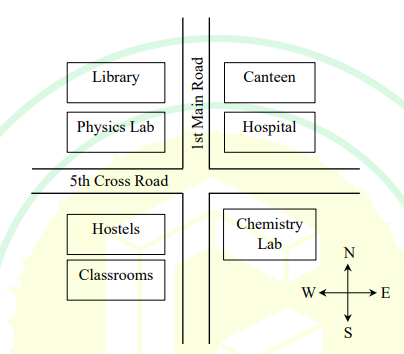
\includegraphics[width=0.6\columnwidth]{figs/Q-5.png}
\caption*{Note:The figure shown is representative}
\label{fig:q5}
\end{figure}

\begin{enumerate}
\item The library is northwest of the canteen
\item The hospital is east of the chemistry lab
\item The chemistry lab is southeast of the physics lab
\item The classrooms and canteen are next to each other
\end{enumerate}
\hfill{\brak{\text{GATE MA 2025}}}

%6
\item “I put the brown paper in my pocket along with the chalks, and possibly other things.
I suppose every one must have reflected how primeval and how poetical are the
things that one carries in one’s pocket: the pocket-knife, for instance the type of all
human tools, the infant of the sword. Once I planned to write a book of poems
entirely about the things in my pocket. But I found it would be too long: and the age
of the great epics is past.”
 \hfill(From G.K. Chesterton’s “A Piece of Chalk”)\\
 
Based only on the information provided in the above passage, which one of the
following statements is true?

\begin{enumerate}
\item The author of the passage carries a mirror in his pocket to reflect upon things.  
\item The author of the passage had decided to write a poem on epics.  
\item The pocket-knife is described as the infant of the sword.  
\item Epics are described as too inconvenient to write.  
\end{enumerate}
\hfill{\brak{\text{GATE MA 2025}}}

%7
\item In the diagram, the lines QR and ST are parallel to each other. The shortest distance
between these two lines is half the shortest distance between the point P and line
QR. What is the ratio of the area of the triangle PST to the area of the trapezium
SQRT?

\begin{figure}[H]
\centering
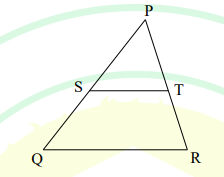
\includegraphics[width=0.5\columnwidth]{figs/Q-7.png}
\caption*{Note:The figure shown is representative}
\label{fig:q7}
\end{figure}

\begin{enumerate}
\begin{multicols}{4}
\item $\tfrac{1}{3}$
\item $\tfrac{1}{4}$
\item $\tfrac{2}{5}$
\item $\tfrac{1}{2}$
\end{multicols}
\end{enumerate}
\hfill{\brak{\text{GATE MA 2025}}}

%8
\item A fair six-faced dice, with the faces labelled ‘1’, ‘2’, ‘3’, ‘4’, ‘5’, and ‘6’, is rolled thrice. What is the probability of rolling ‘6’ exactly once?

\begin{enumerate}
\begin{multicols}{4}
\item $\tfrac{75}{216}$
\item $\tfrac{1}{6}$
\item $\tfrac{1}{18}$
\item $\tfrac{25}{216}$
\end{multicols}
\end{enumerate}
\hfill{\brak{\text{GATE MA 2025}}}

%9
\item A square paper, shown in figure (I), is folded along the dotted lines as shown in the figures (II) and (III). Then a few cuts are made as shown in figure (IV). Which one of the following patterns will be obtained when the paper is unfolded?

\begin{figure}[H]
\centering
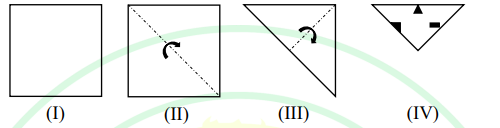
\includegraphics[width=0.8\columnwidth]{figs/Q-9.png}
\caption*{Note:The figure shown are representative}
\label{fig:q9}
\end{figure}


\begin{enumerate}
\item 
\begin{figure}[H]
\centering
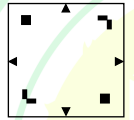
\includegraphics[width=0.2\columnwidth]{figs/Q-9a.png}
\end{figure}  
\item 
\begin{figure}[H]
\centering
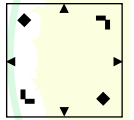
\includegraphics[width=0.2\columnwidth]{figs/Q-9b.png}
\end{figure}
\item 

\begin{figure}[H]
\centering
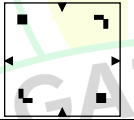
\includegraphics[width=0.2\columnwidth]{figs/Q-9c.png}
\end{figure}
\item 
\begin{figure}[H]
\centering
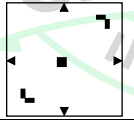
\includegraphics[width=0.2\columnwidth]{figs/Q-9d.png}
\end{figure}
\end{enumerate}
\hfill{\brak{\text{GATE MA 2025}}}

%10
\item A shop has 4 distinct flavors of ice-cream. One can purchase any number of scoops
of any flavor. The order in which the scoops are purchased is inconsequential.
If one wants to purchase 3 scoops of ice-cream, in how many ways can one make
that purchase? 

\begin{enumerate}
\begin{multicols}{4}
\item 4
\item 20
\item 24
\item 48
\end{multicols}
\end{enumerate}
\hfill{\brak{\text{GATE MA 2025}}}

%11
\item Let $S = \cbrak {w = \myvec{w_1\\w_2\\w_3} \in \mathbb{R}^3 \colon \myvec{1&1&1\\-3&1&1\\2&1&1} \myvec{w_1\\w_2\\w_3} \text{ diagonalizable, } \abs{w}=1 }$. Which is true?

\begin{enumerate}
\begin{multicols}{2}
\item $S$ is compact and connected
\item $S$ is neither compact nor connected
\item $S$ is compact but not connected
\item $S$ is connected but not compact
\end{multicols}
\end{enumerate}
\hfill{\brak{\text{GATE MA 2025}}}

%12
\item Given that the Laplace transforms of $J_0(x)$, $J_0'(x)$ and $J_0{''}(x)$ exist, where $J_0(x)$ is the Bessel function. Let $Y = Y(s)$ be the Laplace transform of the Bessel function $J_0(x)$. Then, which one of the following is TRUE?

\begin{enumerate}
\item $\frac{d^Y}{ds} + \frac{2sY}{s^2+1} = 0, s>0$  
\item $\frac{dY}{ds} - \frac{2sY}{s^2+1}=0, s>0$  
\item $\frac{dY}{ds} - \frac{sY}{s^2+1}=0, s>0$  
\item $\frac{dY}{ds} + \frac{sY}{s^2+1} + 1=0, s>0$  
\end{enumerate}
\hfill{\brak{\text{GATE MA 2025}}}

%13
\item To find a real root of the equation $x^3+4x^2-10=0$ in the interval $(1,\frac{3}{2})$ by using the fixed-point iteration scheme, consider the following two statements:

$S_1: x_{k+1}=\sqrt{\tfrac{10}{4+x_k}}, x_0\in \brak{1,\tfrac32}$ converges.  
$S_2: x_{k+1}=\sqrt{10-x_k}$ diverges for some $x_0$ in the same range.

\begin{enumerate}
\item S1 true, S2 false  
\item S2 true, S1 false  
\item Both true  
\item Neither true  
\end{enumerate}
\hfill{\brak{\text{GATE MA 2025}}}

%14
\item For the Linear programming problem: $$\max Z=2x_1+4x_2+4x_3-3x_4$$, 
Subject to $ax_1+x_2+x_3=4, x_1+\beta x_2+x_4=8, x_i\ge0$.

consider the following Statements:  
$S_1:$ If $a=2,\beta=1$, then$(x_1,x_2)^T$ is optimal basis.  
$S_2:$ If $a=1,\beta=4$, then$(x_3,x_2)^T$ is optimal basis.

\begin{enumerate}
\item S1 true, S2 false  
\item S2 true, S1 false  
\item Both true  
\item Neither true  
\end{enumerate}
\hfill{\brak{\text{GATE MA 2025}}}

%15
\item Consider the following subsets of the Euclidean space $\mathbb{R}^4:$
$$S=\{(x_1,x_2,x_3,x_4)\in\mathbb{R}^4\colon x_1^2+x_2^2+x_3^2-x_4^2=0\}$$,  
$$T=\{(x_1,x_2,x_3,x_4)\in\mathbb{R}^4\colon x_1^2+x_2^2+x_3^2-x_4^2=1\}$$, $$U=\{(x_1,x_2,x_3,x_4)\in\mathbb{R}^4\colon x_1^2+x_2^2+x_3^2-x_4^2=-1\}$$. Which is true?

\begin{enumerate}
\item S connected, T,U not  
\item T,U connected, S not  
\item S,U connected, T not  
\item S,T connected, U not  
\end{enumerate}
\hfill{\brak{\text{GATE MA 2025}}}

%16
\item Consider the system of ordinary differential equations
$$\frac{dX}{dt}=MX$$, where $M$ is $6\times 6$ skew-symmetric in $\mathbb{R}$. Then the origin is stable critical point for:

\begin{enumerate}
\begin{multicols}{2}
\item any such matrix $M$
\item only such matrices $M$ whose rank is 2
\item only such matrices $M$ whose rank is 4
\item only such matrices $M$ whose rank is 6
\end{multicols}
\end{enumerate}
\hfill{\brak{\text{GATE MA 2025}}}


% Q.17
\item Let $X = \{ f \in C[0, 1] : f(0) = 0 = f(1)\}$ with the norm $\abs{f}_\infty = \sup_{0 < t \leq 1} \abs{f(t)}$, where $C[0,1]$ is the space of all real-valued continuous functions on $[0,1]$.  
Let $Y = C[0, 1]$ with the norm $\abs{f}_2 = \brak{\int_0^1 \abs{f(t)}^2 dt}^{\tfrac{1}{2}}$.  
Let $U_x$ and $U_y$ be the closed unit balls in $X$ and $Y$ centred at the origin, respectively. Consider $T: X \to \mathbb{R}$ and $S: Y \to \mathbb{R}$ given by  

$Tf = \int_0^1 f(t) dt$ and $Sf = \int_0^1 f(t) dt$.  

Consider the following statements:

S1: $\sup_{f \in U_x} \abs{Tf}$ is attained at a point of $U_x$.  
S2: $\sup_{f \in U_y} \abs{Sf}$ is attained at a point of $U_y$.  

Then, which one of the following is correct?

\begin{enumerate}
\begin{multicols}{2}
\item S1 is TRUE and S2 is FALSE
\item S2 is TRUE and S1 is FALSE
\item both S1 and S2 are TRUE
\item neither S1 nor S2 is TRUE
\end{multicols}
\end{enumerate}  
\hfill{\brak{\text{GATE MA 2025}}}

% Q.18
\item Let $g(x,y) = f(x,y)e^{2x+3y}$ be defined in $\mathbb{R}^2$, where $f(x, y)$ is a continuously differentiable non-zero homogeneous function of degree $4$. Then,  

$$
\frac{\partial g}{\partial x} + \frac{\partial g}{\partial y} = 0
$$  

holds for  

\begin{enumerate}
\begin{multicols}{2}
\item all points $\brak{x,y}$ in $\mathbb{R}^2$
\item all points $\brak{x,y}$ on the line given by $2x + 3y + 4 = 0$
\item all points $\brak{x,y}$ in the region of $\mathbb{R}^2$ except on the line $2x + 3y + 4 = 0$
\item all points $\brak{x,y}$ on the line given by $2x + 3y = 0$
\end{multicols}
\end{enumerate}  
\hfill{\brak{\text{GATE MA 2025}}}

% Q.19
\item The partial differential equation  

$$
\brak{1+x^2}\frac{\partial^2 u}{\partial x^2} + 2x\brak{1-y^2}\frac{\partial^2 u}{\partial y \partial x} + \brak{1-y^2}\frac{\partial^2 u}{\partial y^2} + x\frac{\partial u}{\partial x} + \brak{1-y^2}\frac{\partial u}{\partial y} = 0
$$

is  

\begin{enumerate}
\begin{multicols}{2}
\item elliptic in the region $\{\brak{x,y}\in\mathbb{R}^2 : \abs{y} \leq 1\}$
\item hyperbolic in the region $\{\brak{x,y}\in\mathbb{R}^2 : \abs{y} > 1\}$
\item elliptic in the region $\{\brak{x,y}\in\mathbb{R}^2 : \abs{y} > 1\}$
\item hyperbolic in the region $\{\brak{x,y}\in\mathbb{R}^2 : \abs{y} < 1\}$
\end{multicols}
\end{enumerate}  
\hfill{\brak{\text{GATE MA 2025}}}

% Q.20
\item Let $u(x,t)$ be the solution of the following initial-boundary value problem  

$$
\frac{\partial u}{\partial t} = \frac{\partial^2 u}{\partial x^2}, \quad x \in \brak{0,\pi}, \, t>0,
$$
with $u(0,t) = u(\pi,t) = 0$, $u(x,0) = \sin 4x \cos 3x$.  

Then, for each $t>0$, the value of $u \brak{0,t}$ is  

\begin{enumerate}
\item $\frac{e^{-49t}}{2\sqrt{2}}\brak{e^{48t}-1}$
\item $\frac{e^{-49t}}{2\sqrt{2}}\brak{1-e^{48t}}$
\item $\frac{e^{-49t}}{2\sqrt{2}}\brak{1+e^{48t}}$
\item $\frac{e^{-49t}}{4\sqrt{2}}\brak{1-e^{48t}}$
\end{enumerate}  
\hfill{\brak{\text{GATE MA 2025}}}

% Q.21
\item Consider the function F: R² → R² given by  
$$
F(x,y) = (x³ – 3xy² – 3x,3x²y – y³ – 3y).
$$  
Then, for the function F, the inverse function theorem is  

\begin{enumerate}
\begin{multicols}{2}
\item applicable at all points of R2
\item not applicable at exactly one point of R2
\item not applicable at exactly two points of R2
\item not applicable at exactly three points of R2
\end{multicols}
\end{enumerate}  
\hfill{\brak{\text{GATE MA 2025}}}

% Q.22
\item Let the functions f: R2 → R and g: R2 → R be given by  
$f(x1, x2) = x² + x2 - 2x1x2,$  
$g(x1,x2) = 2x² + 2x² - x_1x_2.$  

Consider the following statements:  
$S_1:$ For every compact subset K of R, $f_{-1}(K)$ is compact.  
$S_2:$ For every compact subset K of R, $g_{-1}(K)$ is compact.  

Then, which one of the following is correct?  

\begin{enumerate}
\begin{multicols}{2}
\item S1 is TRUE and S2 is FALSE
\item S2 is TRUE and S1 is FALSE
\item both S1 and S2 are TRUE
\item neither S1 nor S2 is TRUE
\end{multicols}
\end{enumerate}  
\hfill{\brak{\text{GATE MA 2025}}}

% Q.23
\item Let $pa(x)$ denote the characteristic polynomial of a square matrix $A$. Then, for which of the following invertible matrices $M$, the polynomial $pM(x) — pM_{-1}(x)$ is constant?  

\begin{enumerate}
\begin{multicols}{2}
\item $M = \myvec{3 & 2 \\ 1 & 1}$
\item $M = \myvec{3 & 4 \\ 2 & 2}$
\item $M = \myvec{3 & 1 \\ 0 & 1}$
\item $M = \myvec{3 & 0 \\ 0 & 1}$
\end{multicols}
\end{enumerate}  
\hfill{\brak{\text{GATE MA 2025}}}

% Q.24
\item Consider the balanced transportation problem with three sources S1, S2, S3, and four destinations D1, D2, D3, D4, for minimizing the total transportation cost whose cost matrix is as follows:  

\begin{table}[h!]
\centering
\begin{tabular}{|c|c|c|c|c|c|}
\hline
        & D1 & D2 & D3 & D4 & Supply \\ \hline
S1      & 2  & 6  & 20 & 11 & $\alpha+10$ \\ \hline
S2      & 12 & 7  & 4  & 10 & $\alpha+\lambda+10$ \\ \hline
S3      & 8  & 14 & 16 & 11 & 5 \\ \hline
Demand  & $\alpha+5$ & 10 & $\lambda+5$ & $\alpha+\lambda$ & \\ \hline
\end{tabular}
\caption*{}
\label{tab:q24}
\end{table}  

where $\alpha, \lambda > 0$. If the associated cost to the starting basic feasible solution obtained by using the North-West corner rule is 290, then which of the following is/are correct?  

\begin{enumerate}
\item $\alpha^2 + \lambda^2 = 100$
\item $\alpha^2 + \alpha\lambda = 150$
\item The optimal cost of the transportation problem is 260
\item The optimal cost of the transportation problem is 290
\end{enumerate}  
\hfill{\brak{\text{GATE MA 2025}}}

% Q.25
\item Consider the following regions:  

$S_1 = \{\brak{x_1,x_2}\in \mathbb{R}^2 : 2x_1+x_2 \leq 4, x_1+2x_2 \leq 5, x_1,x_2 \geq 0\},$  

$S_2 = \{\brak{x_1,x_2}\in \mathbb{R}^2 : 2x_1-x_2 \leq 5, x_1+2x_2 \leq 5, x_1,x_2 \geq 0\}.$  

Then, which of the following is/are TRUE?  

\begin{enumerate}
\item The maximum value of $x1+x2$ is 3 on the region S2
\item The maximum value of $x1+x2$ is 5 on the region $S2 - S1$
\item The maximum value of $x1+x2$ is 3 on the region $S1\cap S2$
\item The maximum value of $x1+x2$ is 4 on the region $S1\cup S2$
\end{enumerate}  
\hfill{\brak{\text{GATE MA 2025}}}

% Q.26
\item Let f: R2 – {(0,0)} → R be a function defined by  

$f(x,y) = \dfrac{x^2-y^2}{x^2+y^2} + x \sin\frac{1}{(x^2+y^2)}.$  

Consider the following three statements:  
S1: $\lim_{x \to 0}\lim_{y \to 0} f(x,y)$ exists.  
S2: $\lim_{y \to 0}\lim_{x \to 0} f(x,y)$ exists.  
S3: $\lim_{(x,y)\to(0,0)} f(x,y)$ exists.  

Then, which of the following is/are correct?  

\begin{enumerate}
\begin{multicols}{2}
\item S2 and S3 are TRUE and S1 is FALSE
\item S1 and S2 are TRUE and S3 is FALSE
\item S1 and S3 are TRUE and S2 is FALSE
\item S1, S2 and S3 all are TRUE
\end{multicols}
\end{enumerate}  
\hfill{\brak{\text{GATE MA 2025}}}

% Q.27
\item Let M be a $7 \times 7$ matrix with entries in R and having the characteristic polynomial  
$c_M(x) = (x-1)(x-2)(x-3)^2.$  

Let $\text{rank}(M-I_7) = \text{rank}(M-2I_7) = \text{rank}(M-3I_7) = 5$, where $I_7$ is the $7 \times 7$ identity matrix.  
If $m_M(x)$ is the minimal polynomial of M, then $m_M(5)$ is equal to \underline{\hspace{2cm}} (in integer).  

\hfill{\brak{\text{GATE MA 2025}}}

% Q.28
\item Let $y = P(x)$ be the unique polynomial of degree $n$ satisfying the Legendre differential equation  
\[
(1-x^2)y'' - 2xy' + n(n+1)y = 0,
\]  
and $y(1)=1$.  
Then, the value of $P_{11}(1)$ is equal to \underline{\hspace{2cm}} (in integer).  

\hfill{\brak{\text{GATE MA 2025}}}

% Q.29
\item Let $\mathbf{a}$ be a unit vector parallel to the tangent at the point $P(1,1,\sqrt{2})$ to the curve of intersection of the surfaces $2x^2+3y^2-z^2=3$ and $x^2+y^2=z^2$.  
Then, the absolute value of the directional derivative of $f(x,y,z)=x^2+2y^2-2\sqrt{11}z$ at $P$ in the direction of $\mathbf{a}$ is equal to \underline{\hspace{2cm}} (in integer).  

\hfill{\brak{\text{GATE MA 2025}}}

% Q.30
\item The volume of the region bounded by the cylinders $x^2+y^2=4$ and $x^2+z^2=4$ is equal to \underline{\hspace{2cm}} (rounded off to TWO decimal places).  

\hfill{\brak{\text{GATE MA 2025}}}

% Q.31
\item Let W be the vector space (over R) consisting of all bounded real-valued solutions of the differential equation  
$$
\frac{d^4y}{dx^4} + \frac{d^2y}{dx^2} + y = 0.
$$  
Then, the dimension of W is equal to \underline{\hspace{2cm}} (in integer).  

\hfill{\brak{\text{GATE MA 2025}}}

% Q.32
\item Let $F=(y-z)\mathbf{i}+(z-x)\mathbf{j}+(x-y)\mathbf{k}$ be a vector field, and let S be the surface $x^2+y^2+(z-1)^2=9,$ $1\leq z\leq 4$.  
If $n$ denotes the unit outward normal vector to S, then the value of  
$$
\frac{1}{\pi}\left|\iint_S (\nabla\times F)\cdot n \, dS\right|
$$  
is equal to \underline{\hspace{2cm}} (in integer).  

\hfill{\brak{\text{GATE MA 2025}}}

% Q.33
\item $I = \frac{1}{2\pi i}\int_C \frac{\sin z}{1-\cos(z^3)}dz,$  
where $C = \{z \in C : z= x+iy, |x|+|y|=1, x,y \in R\}$ is oriented positively as a simple closed curve. Then the value of $120I$ is equal to \underline{\hspace{2cm}} (in integer).  

\hfill{\brak{\text{GATE MA 2025}}}

% Q.34
\item Let $\alpha,\beta,\gamma,\delta \in R$ be such that the quadrature formula  
\[
\int_{-1}^1 f(x) dx = \alpha f(-1)+\beta f(1)+\gamma f'(-1)+ \delta f'(1)
\]  
is exact for all polynomials of degree less than or equal to 3.  
Then, $9(\alpha^2+\beta^2+\gamma^2+\delta^2)$ is equal to \underline{\hspace{2cm}} (in integer).  

\hfill{\brak{\text{GATE MA 2025}}}

% Q.35
\item Let $y(x)$ be the solution of the initial value problem  
\[
\frac{dy}{dx} = \sin(\pi(x+y)), \quad y(0)=0.
\]  

Using Euler’s method with step-size $h=0.5$, the approximate value of $y(1.5)+2y(1)$ is equal to \underline{\hspace{2cm}} (in integer).  

\hfill{\brak{\text{GATE MA 2025}}}




% Q.36
\item Consider the linear system $Ax=b$, where $A=[a_{ij}], i,j=1,2,3,$ and $a_{ii}\neq 0$ for $i=1,2,3$, is a matrix with entries in $\mathbb{R}$.  
For 
$$
D=\myvec{A_{11} & 0 & 0 \\ 0 & A_{22} & 0 \\ 0 & 0 & A_{33}},
$$  
let  
$$
D^{-1}A = \myvec{3 & 1 & 2 \\ 1 & 1 & 1 \\ 4 & 0 & 0}, \quad D^{-1}b = \myvec{4 \\ 1 \\ 1}.
$$  

S1: The approximation of $x$ after one iteration of the Jacobi scheme with initial vector $x^{(0)}=\myvec{1 \\ 1 \\ 1}$ is $x_1=\myvec{5 \\ -1 \\ -1}$.  
S2: There exists an initial vector $x^{(0)}$ for which Jacobi iterative scheme diverges.  

Then, which one of the following is correct?  

\begin{enumerate}
\begin{multicols}{2}
\item S1 is TRUE and S2 is FALSE
\item S2 is TRUE and S1 is FALSE
\item both S1 and S2 are TRUE
\item neither S1 nor S2 is TRUE
\end{multicols}
\end{enumerate}
\hfill{\brak{\text{GATE MA 2025}}}

% Q.37
\item Let $y(x)$ be the solution of the differential equation  
$$
x^2y''+7xy'+9y = x^3 \log x, \quad x>0,
$$  
satisfying $y(1)=0$ and $y'(1)=0$.  
Then, the value of $y(e)$ is equal to  

\begin{enumerate}
\begin{multicols}{2}
\item $\dfrac{1}{3}e^{-3}$
\item $\dfrac{1}{6}e^{-3}$
\item $\dfrac{2}{3}e^{-3}$
\item $\dfrac{1}{2}e^{-3}$
\end{multicols}
\end{enumerate}
\hfill{\brak{\text{GATE MA 2025}}}

% Q.38
\item Let $y_1(x)$ and $y_2(x)$ be the two linearly independent solutions of the differential equation  
$$
(1+x^2)y''-xy'+(\cos^2 x)y=0,
$$  
satisfying the initial conditions $y_1(0)=3, y_1'(0)=-1$ and $y_2(0)=-5, y_2'(0)=2$.  

Define $W(x) = \begin{vmatrix} y_1(x) & y_2(x) \\ y_1'(x) & y_2'(x)\end{vmatrix}$.  

Then, the value of $W(1)$ is  

\begin{enumerate}
\begin{multicols}{2}
\item $\tfrac{\sqrt{5}}{4}$
\item $\tfrac{\sqrt{5}}{2}$
\item $\tfrac{2}{\sqrt{5}}$
\item $\tfrac{4}{\sqrt{5}}$
\end{multicols}
\end{enumerate}
\hfill{\brak{\text{GATE MA 2025}}}

% Q.39
\item Let $C$ be the curve of intersection of the surfaces $z^2=x^2+y^2$ and $4x+z=7$.  
If $P$ is a point on $C$ at minimum distance from the $xy$–plane, then the distance of $P$ from the origin is  

\begin{enumerate}
\begin{multicols}{2}
\item $\tfrac{7}{5}$
\item $\tfrac{7\sqrt{2}}{5}$
\item $\tfrac{14}{5}$
\item $\tfrac{14\sqrt{2}}{5}$
\end{multicols}
\end{enumerate}
\hfill{\brak{\text{GATE MA 2025}}}

% Q.40
\item Let $u(x,t)$ be the solution of the initial-value problem  
$$
\frac{\partial^2 u}{\partial t^2} - 9\frac{\partial^2 u}{\partial x^2}=0, \quad x \in \mathbb{R}, \, t>0,
$$  
with initial conditions $u(x,0)=e^x, \; \tfrac{\partial u}{\partial t}(x,0)=\sin x$.  
Then, the value of $u(\pi,\pi)$ is  

\begin{enumerate}
\begin{multicols}{2}
\item $\tfrac{1}{5}(e^\pi+ \sin \pi)$
\item $\tfrac{1}{5}(e^\pi- \sin \pi)$
\item $\tfrac{1}{5}(e^\pi+3)$
\item $\tfrac{1}{5}e^\pi$
\end{multicols}
\end{enumerate}
\hfill{\brak{\text{GATE MA 2025}}}

% Q.41
\item Let $T$ be the Möbius transformation that maps the points $0,i,1$ conformally onto the points $-3,\infty,2$, respectively.  
If $T$ maps the circle centred at $1$ with radius $k$ onto a straight line given by $ax+by+\gamma=0$, then the value of  
$$
\frac{2k(\alpha+\beta)+\gamma}{\alpha+\beta-2k\gamma}
$$  
is equal to  

\begin{enumerate}
\begin{multicols}{2}
\item $\tfrac{1}{7}$
\item $\tfrac{2}{7}$
\item $\tfrac{1}{3}$
\item $\tfrac{2}{13}$
\end{multicols}
\end{enumerate}
\hfill{\brak{\text{GATE MA 2025}}}

% Q.42
\item Let $U=\{z\in\mathbb{C}:\Im(z)>0\}$ and $D=\{z\in \mathbb{C}: \abs{z}<1\}$.  
Let $S$ be the set of all bijective analytic functions $f:U\to D$ such that $f(i)=0$.  
Then, the value of $\sup_{f\in S}\abs{f(4i)}$ is  

\begin{enumerate}
\begin{multicols}{2}
\item $0$
\item $\tfrac{1}{4}$
\item $\tfrac{1}{2}$
\item $\tfrac{3}{5}$
\end{multicols}
\end{enumerate}
\hfill{\brak{\text{GATE MA 2025}}}

% Q.43
\item Let $\Omega$ be a non-empty open connected subset of $\mathbb{C}$ and $f:\Omega\to\mathbb{C}$ a non-constant function. Define $f^2(z)=(f(z))^2, \; f^3(z)=(f(z))^3$.  

S1: If $f$ is continuous in $\Omega$ and $f^2$ is analytic in $\Omega$, then $f$ is analytic in $\Omega$.  
S2: If $f^2$ and $f^3$ are analytic in $\Omega$, then $f$ is analytic in $\Omega$.  

Then, which one of the following is correct?  

\begin{enumerate}
\begin{multicols}{2}
\item S1 is TRUE and S2 is FALSE
\item S2 is TRUE and S1 is FALSE
\item both S1 and S2 are TRUE
\item neither S1 nor S2 is TRUE
\end{multicols}
\end{enumerate}
\hfill{\brak{\text{GATE MA 2025}}}

% Q.44
\item Define on the sphere $S=\{(x_1,x_2,x_3)\in\mathbb{R}^3: x_1^2+x_2^2+x_3^2=1\}$ the relation $(x_1,x_2,x_3)\sim(y_1,y_2,y_3)$ if $x_3=y_3$.  

Let $X=S/\sim$ with quotient topology. Then, which one of the following is TRUE?  

\begin{enumerate}
\begin{multicols}{2}
\item $X$ is homeomorphic to $\{x\in \mathbb{R}: -1\leq x\leq 1\}$
\item $X$ is homeomorphic to $\{(x_1,x_2)\in\mathbb{R}^2: x_1^2+x_2^2=1\}$
\item $X$ is homeomorphic to $\{(x_1,x_2)\in\mathbb{R}^2: x_1^2+x_2^2\leq 1\}$
\item $X$ is homeomorphic to $\{(x_1,x_2,x_3)\in\mathbb{R}^3: x_1^2+x_2^2=1,-1\leq x_3\leq 1\}$
\end{multicols}
\end{enumerate}
\hfill{\brak{\text{GATE MA 2025}}}

% Q.45
\item Consider $X=(C[-1,1],\abs{\cdot}_\infty)$, $Y=(C[-1,1],\abs{\cdot}_2)$ the spaces of continuous functions with sup- and $L^2$-norms.  

Let $W$ be the linear span of all Legendre polynomials.  

Then which of the following is correct?  

\begin{enumerate}
\begin{multicols}{2}
\item $W$ is dense in $X$ but not in $Y$
\item $W$ is dense in $Y$ but not in $X$
\item $W$ is dense in both $X$ and $Y$
\item $W$ is dense neither in $X$ nor in $Y$
\end{multicols}
\end{enumerate}
\hfill{\brak{\text{GATE MA 2025}}}

% Q.46
\item Consider metric spaces $X=(\mathbb{R},d_1), Y=([0,1],d_2)$ with $d_1(x,y)=\abs{x-y}, d_2(x,y)=\abs{x-y}$. Then which is TRUE?  

\begin{enumerate}
\begin{multicols}{2}
\item $[0,1)$ is open in X but not in Y
\item $[0,1)$ is open in Y but not in X
\item $[0,1)$ is open in both X and Y
\item $[0,1)$ is open neither in X nor in Y
\end{multicols}
\end{enumerate}
\hfill{\brak{\text{GATE MA 2025}}}

% Q.47
\item Let $K$ be an algebraically closed field containing a finite field $F$. Let $L$ be the subfield of $K$ consisting of elements of $K$ algebraic over $F$.  

S1: $L$ is algebraically closed.  
S2: $L$ is infinite.  

Which one is correct?  

\begin{enumerate}
\begin{multicols}{2}
\item S1 TRUE, S2 FALSE
\item S2 TRUE, S1 FALSE
\item both TRUE
\item neither TRUE
\end{multicols}
\end{enumerate}
\hfill{\brak{\text{GATE MA 2025}}}

% Q.48
\item Let $M_2(\mathbb{R})$ be the space of $2\times 2$ reals. Define $T(X)=AXB$ with matrices  

$A=\myvec{1 & -4 \\ 6 & -2}, \; B=\myvec{5 & 0 \\ -1 & -1}.$  

Let $P$ be the representation matrix of $T$. Which of the following are TRUE?  

\begin{enumerate}
\item P is invertible
\item The trace of P is 25
\item The rank of $(P^2-4I_4)$ is 4
\item The nullity of $(P-2I_4)$ is 0
\end{enumerate}
\hfill{\brak{\text{GATE MA 2025}}}

% Q.49
\item Consider the LPP: Maximize $Z=3x_1+5x_2$ subject to $x_1+x_3=4, 2x_2+x_4=12, 3x_1+2x_2+x_5=18, x_i\geq 0$.  

Given that $(x_3,x_2,x_1)$ is optimal basis with $B^{-1}=\myvec{\alpha & -\beta & \beta \\ \gamma & 0 & 0 \\ 1 & 0 & 0}$.  

If $(p,q,r)$ is optimal dual solution, which are TRUE?  

\begin{enumerate}
\item $\alpha+3\beta+2\gamma=3$
\item $\alpha-3\beta+4\gamma=1$
\item $p+q+r=\tfrac{5}{2}$
\item $p^2+q^2+r^2=\tfrac{17}{4}$
\end{enumerate}
\hfill{\brak{\text{GATE MA 2025}}}

% Q.50
\item Let $0<\alpha<1$. Define  
$$
C^\alpha[0,1]=\{f:[0,1]\to\mathbb{R}: \sup_{s\neq t}\frac{\abs{f(t)-f(s)}}{\abs{t-s}^\alpha}<\infty\}.
$$  
This is Banach under norm $\abs{f}_\alpha=\abs{f(0)}+\sup_{s\neq t}\frac{\abs{f(t)-f(s)}}{\abs{t-s}^\alpha}$.  

Let $C[0,1]$ with sup norm. Define $T:C^\alpha[0,1]\to C[0,1], Tf=f$. Then:  

\begin{enumerate}
\item $T$ is a compact linear map
\item Image of T is closed
\item Image of T is dense
\item T is not bounded
\end{enumerate}
\hfill{\brak{\text{GATE MA 2025}}}

% Q.51
\item PDE: $\tfrac{\partial u}{\partial t}+3\tfrac{\partial u}{\partial x}=u, \; u(x,0)=\cos x$. Let $v$ satisfy $\tfrac{\partial v}{\partial t}+3\tfrac{\partial v}{\partial x}=v^2, \; v(x,0)=\cos x$.  

Which are TRUE?  

\begin{enumerate}
\item $\abs{u(x,t)}\leq e^t$ for all $x,t$
\item $v(x,1)$ not defined for some $x$
\item $v(x,1)$ not defined for any $x$
\item $u(2\pi,\pi)=-e^\pi$
\end{enumerate}
\hfill{\brak{\text{GATE MA 2025}}}

% Q.52
\item Heat equation $\tfrac{\partial u}{\partial t}=2\tfrac{\partial^2 u}{\partial x^2}, 0<x<1,t>0$; $u(0,t)=u(1,t)=0, u(x,0)=2x(1-x)$.  

Which are TRUE?  

\begin{enumerate}
\item $0\leq u(x,t)\leq 1/4$ all $x,t$
\item $u(x,t)=u(1-x,t)$
\item $\int_0^1 u(x,t)^2dx$ decreasing in $t$
\item Same integral not decreasing
\end{enumerate}
\hfill{\brak{\text{GATE MA 2025}}}

% Q.53
\item $f(x,y)=(e^{2\pi x}\cos 2\pi y, e^{2\pi x}\sin 2\pi y)$. Which are TRUE?  

\begin{enumerate}
\item If G open, then f(G) open
\item If G closed, then f(G) closed
\item If G dense, f(G) dense
\item f is surjective
\end{enumerate}
\hfill{\brak{\text{GATE MA 2025}}}

% Q.54
\item Let $\{x_k\}$ orthonormal in Hilbert space X. For fixed n, let $Y=\text{span}\{x_1,\dots,x_n\}$. Define $S_n(x)=\sum_{k=1}^n \langle x,x_k\rangle x_k$. Then:  

\begin{enumerate}
\item $S_n(x)$ is orthogonal projection on Y
\item $S_n(x)$ is projection on $Y^\perp$
\item $x-S_n(x)\perp S_n(x)$
\item $\sum_{k=1}^n\abs{\langle x,x_k\rangle}^2=\abs{x}^2$ for all x
\end{enumerate}
\hfill{\brak{\text{GATE MA 2025}}}

% Q.55
\item Sequence $f_1(x)=x/2$, $f_{n+1}(x)=f_n(x)-\tfrac12(f_n(x)^2-x)$. Then:  

\begin{enumerate}
\item pointwise but not uniform convergence
\item uniform convergence
\item $\sqrt{x}-f_n(x)> \tfrac{2\sqrt{x}}{2+n\sqrt{x}}$
\item $0\le f_n(x)\le \sqrt{x}$
\end{enumerate}
\hfill{\brak{\text{GATE MA 2025}}}

% Q.56
\item $u_n(x)=\sin(nx)/\sqrt{n}, x\in(0,\pi)$. Then:  

\begin{enumerate}
\item $\sum u_n$ converges uniformly
\item $\sum u_n$ converges uniformly
\item converges pointwise not uniform
\item converges uniformly on compacts
\end{enumerate}
\hfill{\brak{\text{GATE MA 2025}}}

% Q.57
\item Let $S^1=\{(x_1,x_2)\in\mathbb{R}^2:x_1^2+x_2^2=1\}$. For continuous non-constant $f:S^1\to\mathbb{R}$:  

\begin{enumerate}
\item maps closed sets to closed
\item is injective
\item is surjective
\item $\exists \lambda: f(\cos\lambda,\sin\lambda)=f(-\cos\lambda,-\sin\lambda)$
\end{enumerate}
\hfill{\brak{\text{GATE MA 2025}}}

% Q.58
\item Let X uncountable set with co-countable topology. Then:  

\begin{enumerate}
\item compact subset closed
\item closed subset compact
\item X is T1 not T2
\item X is T2
\end{enumerate}
\hfill{\brak{\text{GATE MA 2025}}}

% Q.59
\item Statements about commutative rings:  

P1: R is isomorphic to $R_1\times R_2$  
P2: $\exists r_1,r_2$ with $r_1^2=r_1\neq 0, r_2^2=r_2\neq 0, r_1r_2=0, r_1+r_2=1$  
P3: $\exists I_1,I_2$ ideals, $R=I_1+I_2, I_1\cap I_2=0$  
P4: $\exists a,b\neq0$ with $ab=0$  

Which are TRUE?  

\begin{enumerate}
\item P1 $\Leftrightarrow$ P2
\item P2 $\Rightarrow$ P3
\item P3 $\Rightarrow$ P4
\item P4 $\Rightarrow$ P1
\end{enumerate}
\hfill{\brak{\text{GATE MA 2025}}}

% Q.60
\item Let extensions $E\subset F\subset K$ not algebraic. Let $a\in K$ algebraic over $F$, not in $F$. Let $L$ be subfield of $K$ generated over $E$ by coefficients of minimal polynomial of a over $F$. Then:  

\begin{enumerate}
\item $F(a)\supset L(a)$ finite $\Leftrightarrow F\supset L$ finite
\item $\dim L(a)/L > \dim F(a)/F$
\item $\dim L(a)/L < \dim F(a)/F$
\item $F(a)\supset L(a)$ alg. $\Leftrightarrow F\supset L$ alg.
\end{enumerate}
\hfill{\brak{\text{GATE MA 2025}}}

% Q.61
\item Inner product $(f,g)=\int_{-1}^1 f(x)g(x) dx$.  

If $p(x)=\alpha+\beta x^2-30x^4$ is orthogonal to all polynomials degree $\le 3$, then $\alpha+5\beta$ is equal to \underline{\hspace{2cm}} (in integer).  
\hfill{\brak{\text{GATE MA 2025}}}

% Q.62
\item For $X=\myvec{x_1 \\ x_2 \\ x_3}$, quadratic form  
$$
Q(X)=2x_1^2+2x_2^2+3x_3^2+4x_1x_2+2x_1x_3+2x_2x_3.
$$  
Let M be symmetric matrix of Q. For $Y\in\mathbb{R}^3$ non-zero define  
$$
a_n=\frac{Y^T(M+I_3)^{n+1}Y}{Y^T(M+I_3)^nY}, \, n=1,2,...
$$  
Then $\lim_{n\to\infty}a_n=$ \underline{\hspace{2cm}} (in integer).  
\hfill{\brak{\text{GATE MA 2025}}}

% Q.63
\item Let $\alpha,\beta$ distinct nonzero reals, Q(z) polynomial deg<5. If  
$$
f(z)=\frac{\alpha^6\sin(\beta z)-\beta^6(e^{2\alpha z}-Q(z))}{z^6}
$$  
satisfies Morera in $\mathbb{C}\setminus\{0\}$, then $\tfrac{\alpha}{4\beta}=$ \underline{\hspace{2cm}}.  
\hfill{\brak{\text{GATE MA 2025}}}

% Q.64
\item Let G group with $g,h\in G$, $g\neq e,g^2=e,h\neq e,h^2\neq e, ghg^{-1}=h^2$. Then, least positive n with $h^n=e$ is \underline{\hspace{2cm}}.  
\hfill{\brak{\text{GATE MA 2025}}}

% Q.65
\item Let $(\mathbb{R}^2,d_1),(\mathbb{R}^2,d_2)$ be metric spaces with  
$$
d_1((x_1,x_2),(y_1,y_2))=\abs{x_1-y_1}+\abs{x_2-y_2},
$$  
$$
d_2((x_1,x_2),(y_1,y_2))=\frac{d_1((x_1,x_2),(y_1,y_2))}{1+d_1((x_1,x_2),(y_1,y_2))}.
$$  
If the open ball centred at $(0,0)$ with radius $1/\alpha$ in $(\mathbb{R}^2,d_1)$ equals the ball with radius $1/7$ in $(\mathbb{R}^2,d_2)$, then $\alpha=$ \underline{\hspace{2cm}}.  
\hfill{\brak{\text{GATE MA 2025}}}



\end{enumerate}
\end{document}
